
%PRIMA SBOBINA DI ORTOPEDIA

\section{Le scoliosi}

\subsection{Definizione }


\emph{Le \textbf{scoliosi} è una patologia relativamente frequente in
ambito ortopedico in particolar modo la scoliosi secondaria idiopatica
ha un'elevata incidenza in ambito pediatrico ed è gravata da una molte
false credenze non supportate da solide prove scientifiche.}

Per \textbf{scoliosi} intendiamo una \emph{deviazione del rachide sul
piano frontale.} Normalmente la colonna vertebrale vista dal davanti
deve essere dritta mentre in caso di scoliosi c'è tale deviazione sul
piano frontale che si apprezza come una curva non fisiologica

È molto importante distinguere fin da subito tra:

\begin{itemize}
\item
  \textbf{\emph{Scoliosi vere}} o \textbf{\emph{Scoliosi strutturate}} o
  \textbf{\emph{Scoliosi organiche}} definite propriamente come
  deformità del rachide
\item
  \textbf{\emph{Scoliosi finte}} o \textbf{\emph{atteggiamenti
  scoliotici}} riconducibili a ben precise cause che una volta rimosse
  permettono la risoluzione della deviazione sul piano frontale.
\end{itemize}

Alla luce di quanto detto solo le \textbf{\emph{scoliosi vere}} sono
considerate come vere e proprie patologie dal punto di vista ortopedico

\subsection{Atteggiamento scoliotico}


L'atteggiamento scoliotico è una \textbf{\emph{deviazione laterale del
rachide}} che presenta alcuni segni clinici comuni alla scoliosi vera
(strutturata):

\begin{itemize}
\item
  Asimmetria delle creste iliache
\item
  Asimmetria delle spalle
\item
  Asimmetria delle anche.
\end{itemize}

L'atteggiamento scoliotico (la cosiddetta ``curva finta'') non presenta
invece i \textbf{fenomeni di} \textbf{strutturazione} tipici della
scoliosi vera ossia la \textbf{deformità dei corpi vertebrali} da cui la
mancanza \textbf{dell'asimmetria del torace} o \textbf{gibbo costale}
quando il rachide è flesso

N.B- Dal punto di vista clinico il gibbo costale è l'aspetto più
importante e caratteristico delle scoliosi vere.

\subsubsection{Eziologia}


L'\textbf{atteggiamento scoliotico} può essere dovuto a moltissime
cause:

\begin{enumerate}
\def\labelenumi{\arabic{enumi}.}
\item
  \textbf{Eterometria degli arti inferiori:} si definisce così la
  condizione in cui i due arti non presentano la stessa lunghezza per
  cui il bacino risulta inclinato. C'è un tentativo di compenso
  sovra-segmentario da parte della colonna vertebrale attraverso una
  flessione sul piano frontale. \emph{Una dismetria è considerata
  normale fino a 1.5 cm ed è compensata dalla scoliosi}
\item
  \textbf{Contrattura antalgica:} una coxalgia acuta (dolore improvviso
  all'anca) determina una contrattura dei muscoli e quindi la
  possibilità che il bacino si inclini: ciò provocherà alla fine una
  curvatura della colonna sul piano frontale.
\item
  \textbf{Posturale:} una postura scorretta che prima o poi produce una
  modesta curva sul piano frontale. Può diventare anche dolente perché i
  muscoli vanno in tensione, ma \emph{non} sono di fronte a una
  \emph{scoliosi vera}! L'atteggiamento scoliotico di tipo posturale è
  un qualcosa che una volta risolta la contrattura, anche attraverso una
  ginnastica postulare, scompare.
\begin{quote}
N.B. La ginnastica posturale non è indicata tanto meno utile nella
scoliosi strutturale che è una deformità.
\end{quote}
\item
  \textbf{Isterica:} l'isterismo è una malattia psichiatrica che mima
  moltissime malattie e può mimare anche una scoliosi.
\item
  \textbf{Irritazione delle radici nervose}: ernia del disco, tumori,
  metastasi, ecc.
\begin{quote}
Esempio classico è quello \emph{dell'ernia del disco (e.d.d.)}: chi ha
una e.d.d. sviluppa una \emph{scoliosi di tipo antalgico} nel tentativo
di sentire meno dolore: quando ho una compressione da parte dell'ernia
sulla radice nervosa, il tentativo inconscio del corpo umano è quello di
dare un po' più spazio a questa radice per ridurre la compressione. Una
volta che va via l'infiammazione della radice oppure togliamo l'ernia,
l'atteggiamento scoliotico di flessione laterale del tronco viene meno
perché non c'è più l'irritazione.

Altro esempio\emph{:} una \emph{metastasi.} La metastasi può dare
compressione o irritazione della radice e produrre un atteggiamento
scoliotico.
\end{quote}

\item
  \textbf{Infiammatoria}: appendicite, patologie renali, gastriche, ecc.


\begin{quote}
Un\emph{'appendicite acuta} può determinare una contrazione dei muscoli
della parete addominale e ciò può produrre un atteggiamento scoliotico.

Patologie renali\emph{:} anche una \emph{colica renale} può determinare
una contrattura dei muscoli della parete addominale e dare un
atteggiamento scoliotico.
\end{quote}
\end{enumerate}
\paragraph{1. ETEROMETRIA DEGLI ARTI INFERIORI.}
\begin{figure}[!ht]
\centering
	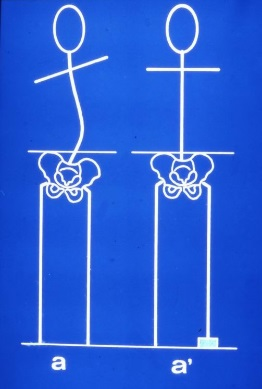
\includegraphics[width=0.5\textwidth]{012/image1.jpeg}
\end{figure}

Nello schema ``\textbf{a}'' l'arto inferiore di sinistra è più corto e
ciò determina la ``caduta'' (inclinazione verso il basso) del bacino
dallo stesso lato. La conseguenza è che si viene a creare una curva
della colonna vertebrale a livello lombare.

In ``\textbf{a'}'' viene messo un rialzo al di sotto dell'arto più corto
(si compensa la dismetria) e la scoliosi finta scompare. Si tratta
propriamente di un atteggiamento scoliotico che scompare una volta
trattata la causa primaria che nell'esempio è la dismetria.

\paragraph{2. CONTRATTURA O DEFORMITÀ DELL'ANCA. }


\begin{figure}[!ht]
\centering
	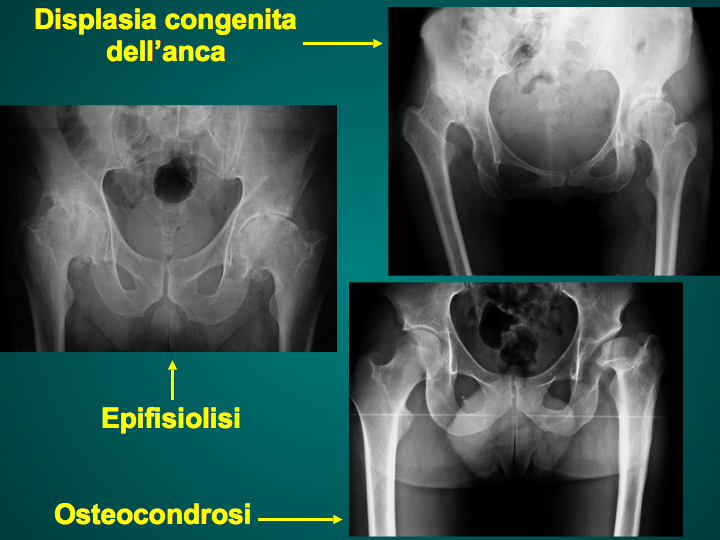
\includegraphics[width=0.5\textwidth]{012/image2.png}
\end{figure}

Altre condizioni che abbiamo detto poter determinare una scoliosi finta o
atteggiamento scoliotico sono le deformità a livello dell'anca.

\begin{enumerate}
\def\labelenumi{\arabic{enumi}.}
\item
  \textbf{DISPLASIA O LUSSAZONE CONGENITA DELL'ANCA.} Nella radiografia
  si apprezza la lussazione: la testa di un femore è dislocata più in
  alto rispetto alla testa dell'altro (tipico esempio di lussazione
  inveterata dell'anca su base congenita). Ciò comporta un accorciamento
  dell'arto corrispondente e quindi l'innesco di una curva scoliotica.
\item
  \textbf{OSTEOCONDROSI:} Coxa plana come esito di osteocondrosi
  (necrosi del nucleo di accrescimento della testa del femore): si ha un
  accorciamento dell'arto inferiore corrispondente e ciò a sua volta
  innesca una curva scoliotica ``finta''.
\end{enumerate}

\paragraph{3. SCOLIOSI POSTURALE.}


Ci sono diverse posture scorrette (determinate anche da situazioni di
tipo psicologico) che possono portare all'innesco di una curva con segni
che possono ricordare quelli di una deformità vera, ma in realtà non
sono sostenuti da \emph{fenomeni di strutturazione} che sono gli
elementi che caratterizzano la scoliosi vera.

Utile in questi casi è osservare il paziente in flessione anteriore
perché nella scoliosi posturale non ci sarà alcuna differenza tra i due
emitoraci ovvero non ci sarà il gibbo costale.

\paragraph{4. SCOLIOSI ISTERICA.}


La paziente raffigurata, affetta da isterismo, ha assunto questo
atteggiamento.

\begin{figure}[!ht]
\centering
	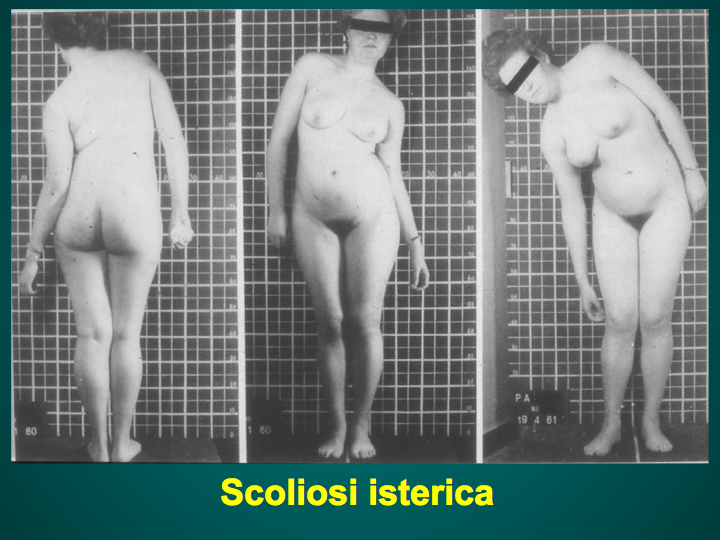
\includegraphics[width=0.5\textwidth]{012/image3.png}
\end{figure}

Il problema di base non è la scoliosi! Si ha un atteggiamento scoliotico
(una curva sul piano frontale) dovuta all'isterismo. La somministrazione
di Valium potrebbe essere sufficiente per risolvere questa condizione
posturale.

\begin{figure}[!ht]
\centering
	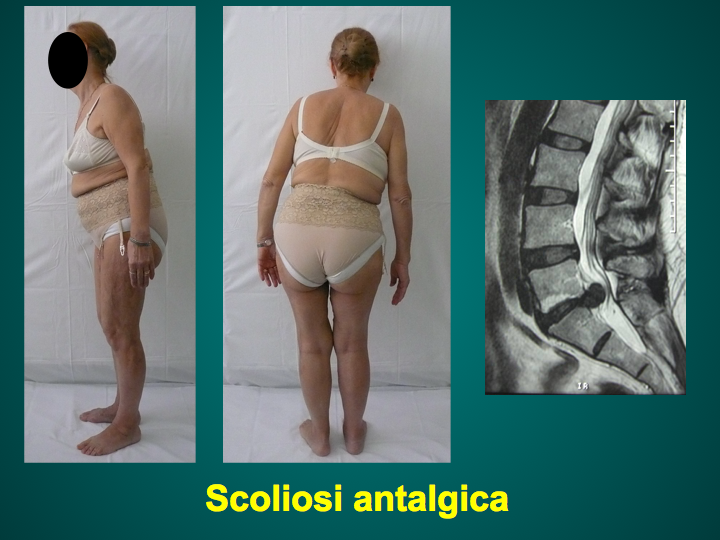
\includegraphics[width=0.5\textwidth]{012/image4.png}
\end{figure}

\paragraph{5.SCOLIOSI ANTALGICA.}


La risonanza magnetica mette in evidenza un'\emph{ernia del disco} (il
nucleo del disco intervertebrale è erniato posteriormente e determina
una compressione delle radici nervose a livello di L5-S1). Si ha innesco
di una sintomatologia dolorosa (lombalgia = sintomatologia centrale;
lombo sciatalgia = sintomatologia periferica) e l'individuo assume
questo atteggiamento detto antalgico nel tentativo di alleviare il
dolore. La somministrazione di cortisone o di un antidolorifico può
essere sufficiente per risolvere questo atteggiamento postulare.

\subsubsection{Terapia}


L'\textbf{atteggiamento scoliotico} è un qualcosa che \textbf{viene meno
nel momento in cui si} \textbf{rimuove la causa} perciò non sono
necessarie forme di trattamento come quelle che invece vengono adottate
in caso di \emph{scoliosi vera}.

\begin{itemize}
\item
  L'unico trattamento è \textbf{\emph{rimuovere la causa}}
  dell'atteggiamento scoliotico

  \textbf{\emph{Non}} sono \textbf{\emph{necessarie}} ginnastica
  correttiva, nuoto correttivo, elettrostimolazioni ecc.
\end{itemize}

\subsection{Scoliosi strutturata (organica)}

\subsubsection{Definizione}


La \textbf{scoliosi vera} (detta anche \textbf{strutturata o organica})
è propriamente una \textbf{deformità del rachide.}

N.B. Per deformità in ambito ortopedico intendiamo (in modo generico!)
tutte quelle \emph{situazione che il soggetto non può correggere
volontariamente.}

L'\emph{atteggiamento scoliotico} non è una deformità in quanto
\emph{può essere corretto volontariamente}.

Un \emph{piede torto, una scoliosi} (e qualsiasi altra deformità) invece
\emph{non possono essere corrette volontariamente dal soggetto.}

Definiamo la \textbf{scoliosi vera} come una \emph{deviazione laterale e
permanente del rachide sul piano frontale associata a fenomeni
\textbf{``di strutturazione''} dei corpi}
\emph{vertebrali}.

\begin{figure}[!ht]
\centering
	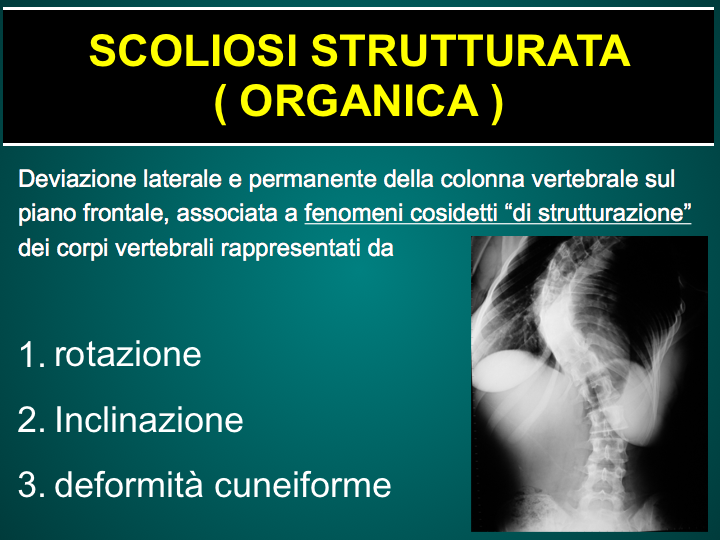
\includegraphics[width=0.5\textwidth]{012/image5.png}
\end{figure}

I \emph{\textbf{Fenomeni di strutturazione}} che connotano la scoliosi
vera sono:

\begin{enumerate}
\def\labelenumi{\arabic{enumi}.}
\item
  \textbf{Rotazione delle vertebre};
\item
  \textbf{Inclinazione delle vertebre};
\item
  Deformità cuneiforme che il professore preferisce definire come
  \emph{\textbf{deformità trapezoidale}} in quanto valutando la forma
  della vertebra nella radiografia, si vede che la vertebra dalla parte
  della concavità della curva risulta più bassa mentre dalla parte della
  convessità risulta più alta. Questo è dovuto al fatto che un osso se
  sottoposto a una pressione maggiore si sviluppa di meno.
\item
  Nella diapositiva non compare un quarto fenomeno di strutturazione
  perché ritenuto dal professore un fenomeno ``super specialistico''
  \emph{ovvero la \textbf{Torsione della vertebra: }}la rotazione della
  vertebra si associa anche ad una torsione della vertebra stessa.
\end{enumerate}

Questi sono alla base di ciò che noi vediamo clinicamente come ad
esempio il \textbf{gibbo costale} o la \textbf{prominenza lombare}.

Se non ci sono questi fenomeni di strutturazione (visibili sia
clinicamente che radiograficamente) non possiamo parlare di scoliosi
organica.

Gli ortopedici lavorano prevalentemente sulle scoliosi vere e non
sull'atteggiamento scoliotico dal momento che in questo secondo caso non
si ha deformità e non è necessario intervenire con trattamenti
chirurgici o con busti. Dal punto di vista ortopedico il primo approccio
è quello di valutare se ci si trova di fronte a una scoliosi vera o a un
atteggiamento scoliotico e nel caso in cui ci si trovi davanti ad una
scoliosi vera si deve intervenire per correggere e evitarne il
peggioramento.

\subsubsection{Epidemiologia}


\begin{figure}[!ht]
\centering
	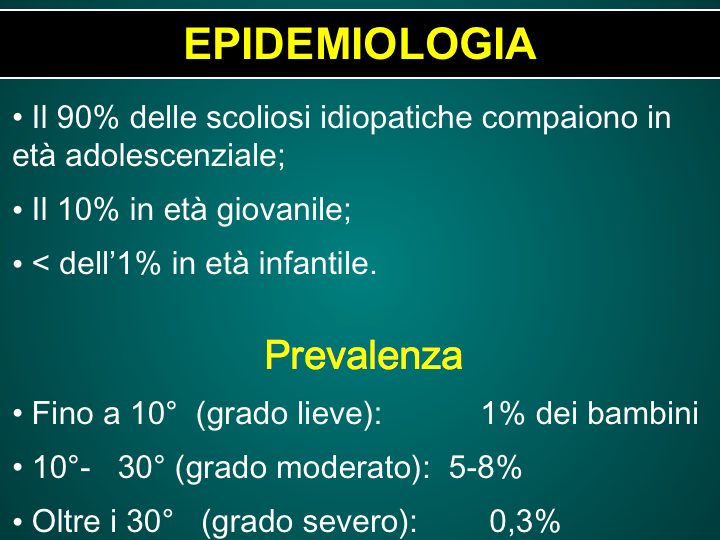
\includegraphics[width=0.5\textwidth]{012/image6.png}
\end{figure}

\emph{(Queste cose si mettono per completezza, ma in realtà non hanno molto senso dal
momento che i lavori di tipo epidemiologico risentono di tante
cose\ldots{} L'epidemiologia di dove? Dell'Italia? Del Canada? Degli
Stati Uniti? Ovviamente lì si risente anche di situazioni geografiche,
si risente di situazioni anche razziali quindi obiettivamente sono
numeri che presi in sé e per sé non hanno molta importanza\ldots{} Ci
servono grosso modo e vengono dati a lezione per vedere un po' la
grandezza del problema)} In Italia l'incidenza di scoliosi vere è
piuttosto elevata però \emph{\textbf{quelle da curare} \textbf{sono
pochissime}. Quindi la dimensione del problema è un po' questa.}
Probabilmente insieme al piede piatto la scoliosi è la prima (se non la
seconda) causa di consultazione dell'ortopedico da parte dei pazienti e
delle famiglie.

\emph{Dal punto di vista epidemiologico:}

\begin{itemize}
\item
  \emph{Il 90\% delle scoliosi compare in \emph{età adolescenziale}: tra
  gli 8 ed i 10 anni}
\item
  \emph{Il 10\% in \emph{età giovanile}}
\item
  \emph{Solo l'1\% in \emph{età infantile}. }
\end{itemize}

\emph{La scoliosi vera può essere poi classificata in diversi gradi in
base all'angolo di curvatura della colonna: }

\begin{itemize}
\item
  \emph{Con angoli fino a 10\textsuperscript{o} si parla di scoliosi \textbf{lieve} che ha
  peraltro una prevalenza dell'1\%, }
\item
  \emph{Con angoli tra 10\textsuperscript{o} e 30\textsuperscript{o} si ha una scoliosi \textbf{moderata}
  che ha una prevalenza tra il 5 e l'8\%}
\item
  \emph{Con angoli oltre i 30\textsuperscript{o} è giustificato l'uso del termine scoliosi
  \textbf{severa} che ha fortunatamente una prevalenza solo dello
  0,3\%.}
\end{itemize}

\subsubsection{Eziologia e classificazione delle scoliosi}

\begin{figure}[!ht]
\centering
	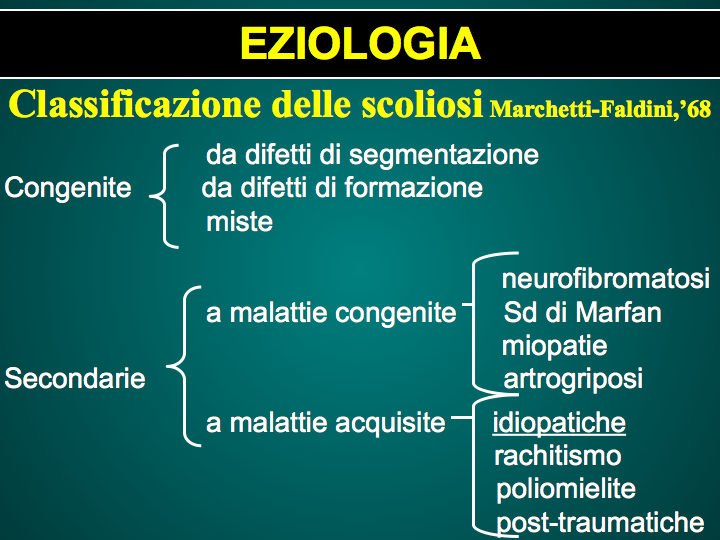
\includegraphics[width=0.5\textwidth]{012/image7.png}
\end{figure}

Di classificazioni ce ne sono molte, ma il professore riporta sempre questa
perché dice di aver avuto l'onore di lavorare con i proff. Marchetti e
Faldini che nel 1968 fecero questa classificazione molto semplice.

Il vantaggio di questa classificazione deriva dal fatto che comprende la
famiglia delle \textbf{\emph{scoliosi idiopatiche}}: scoliosi delle
quali non conosciamo la causa e che sono quelle di maggiore incidenza
nelle bambine e nei bambini attorno agli 8-10 anni.

Le scoliosi idiopatiche saranno il centro di questa lezione perché
quando ci si trova di fronte ad un paziente affetto da neurofibromatosi
(\emph{``di Recklinghausen''}) o da distrofia muscolare (\emph{``di
Duchenne''}, bambini che muoiono all'età di 10-12 anni perché non
respirano più) la scoliosi è il problema minore.

\emph{Le scoliosi che vanno a finire male sono quelle poche scoliosi
idiopatiche che vengono sottovalutate mentre le poche scoliosi
idiopatiche che tendono a peggiorare sono poi quelle che sfuggono e che
costringono a interventi chirurgici molto impegnativi} (incisioni di 80
cm - 1 m a livello della schiena e barre di titanio).

Le scoliosi vengono suddivise in 2 grandi famiglie:

\begin{enumerate}
\def\labelenumi{\arabic{enumi}.}
\item
  \textbf{SCOLIOSI CONGENITE} (o primitive) così dette perché la causa
  risiede nella colonna vertebrale e ulteriormente suddivise in:

\begin{enumerate}
\def\labelenumi{\arabic{enumi}.}
\item
  \emph{Scoliosi da difetti di segmentazione};

  \emph{Scoliosi da difetti di formazione};

  \emph{Scoliosi miste}.
\end{enumerate}


\item
  \textbf{SCOLIOSI SECONDARIE}, a loro volta suddivise in

\begin{enumerate}
\def\labelenumi{\arabic{enumi}.}
\item
  SCOLIOSI SECONDARIE A MALATTIE CONGENITE:

\begin{enumerate}
\def\labelenumi{\arabic{enumi}.}
\item
  \emph{Neurofibromatosi};
\item 
  \emph{Sindrome di Marfan};
\item 
  \emph{Miopatie};
\item 
  \emph{Artrogriposi}.
\end{enumerate}


\item
  SCOLIOSI SECONDARIE A MALATTIE ACQUISITE:

\begin{enumerate}
\def\labelenumi{\arabic{enumi}.}
\item
  \emph{Scoliosi post-traumatiche}: una frattura che causa un
  abbassamento di 2 corpi vertebrali a sinistra, determinerà una
  scoliosi
\item
  \emph{Poliomielite}: malattia virale causata da un enterovirus
  caratterizzato da uno spiccato neurotropismo. Si avrà un'alterazione
  dell'equilibrio muscolare con azione sulla colonna vertebrale e questo
  innescherà una scoliosi: la poliomielite è una paralisi flaccida
\item
  \emph{Rachitismo};
\end{enumerate}
\end{enumerate}
\item
  \emph{\textbf{\emph{Scoliosi idiopatiche:}}} vengono considerate
  secondarie a qualcosa che non conosciamo (non conoscendo la causa
  vengono definite idiopatiche, ma sono comunque secondarie a qualcosa).
  Qual è il problema? È un po' quello che accade con una febbre che di
  giorno in giorno cresce fino ad arrivare a valori critici. Se non
  riesco a trovare la causa (polmonite? appendicite?) cerco comunque di
  intervenire per curare il sintomo (la febbre). Nel caso delle scoliosi
  idiopatiche ci troviamo nella stessa situazione! Non conosciamo la
  causa, ma il sintomo (la curva della colonna vertebrale) che può
  peggiorare e acquisire i caratteri di malattia perciò occorrerà
  trattare il sintomo (la scoliosi) pur non conoscendo (a oggi) la
  causa.

\end{enumerate}

Solitamente, quando alla base della scoliosi si ha una malattia
congenita o acquisita grave i casi non sfuggono all'osservazione.
Bisogna stare attenti invece a tutti gli altri casi che possono
sfuggire.

Le scoliosi idiopatiche sono moltissime, ma quelle da curare sono
pochissime. Il problema sarà \textbf{individuarle} e \textbf{capirle}:
capire se ci si trova davanti a una forma che tende a peggiorare nel
tempo e a diventare grave oppure se si tratta di una scoliosi modesta
che non andrà incontro a peggioramento. \emph{Non essendo nota la causa
non possiamo fare una prognosi e non possiamo sapere quale sarà
l'evoluzione. }

\paragraph{SCOLIOSI CONGENITE}


Le scoliosi congenite sono \textbf{dovute ad anomalie di sviluppo della
colonna vertebrale:}

\begin{enumerate}
\def\labelenumi{\arabic{enumi}.}
\item
  \textbf{DIFETTI DI FORMAZIOINE}...Si formano ``mezze vertebre'': gli
  \textbf{emispondili.} Nell'immagine in basso a dx si vede come
  l'emispondilo crea una sorta di cuneo: le curve sono molto strette,
  molto piccole e comprendono poche vertebre.
\item
  \textbf{DIFETTI DI SEGMENTAZIONE}... Non si separano i corpi
  vertebrali: \textbf{sinostosi} ed è come se le vertebre fossero fuse,
  ma in realtà quello che si ha è una mancata separazione. Nell'immagine
  in basso a destra è riportata una \emph{stratigrafia:} è una forma di
  radiografia fatta con un tubo radiogeno che si muove e consente di
  ottenere una ``fetta'' di TAC. Ciò che si vede nella stratigrafia è
  che 3 o 4 vertebre sono interessate da questa ``mancata segmentazione
  ``che porta ad una fusione.
\item
  \textbf{MISTE}: si ha un'associazione tra emispondili e mancate
  separazioni. Le forme miste sono quelle più frequenti.
\end{enumerate}

\begin{figure}[!ht]
\centering
	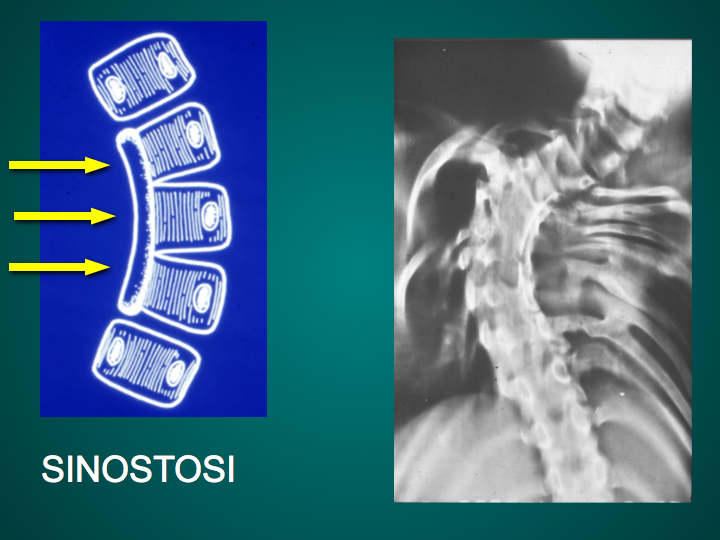
\includegraphics[width=0.5\textwidth]{012/image8.png}
\end{figure}
\begin{figure}[!ht]
\centering
	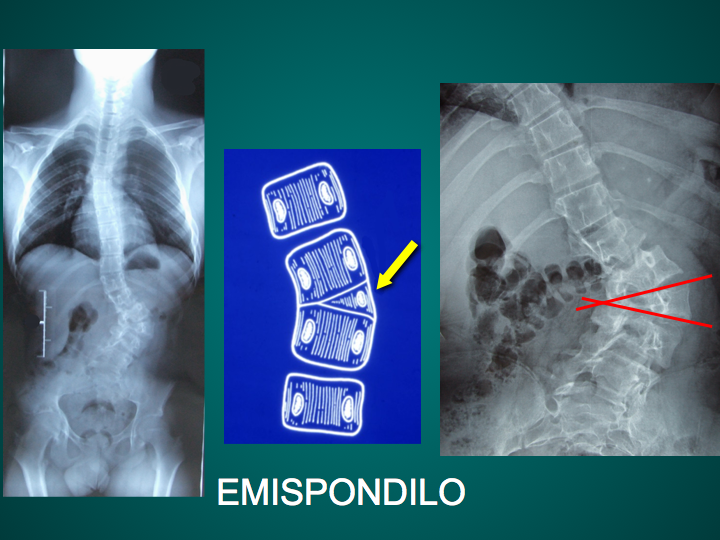
\includegraphics[width=0.5\textwidth]{012/image9.png}
\end{figure}
\begin{figure}[!ht]
\centering
	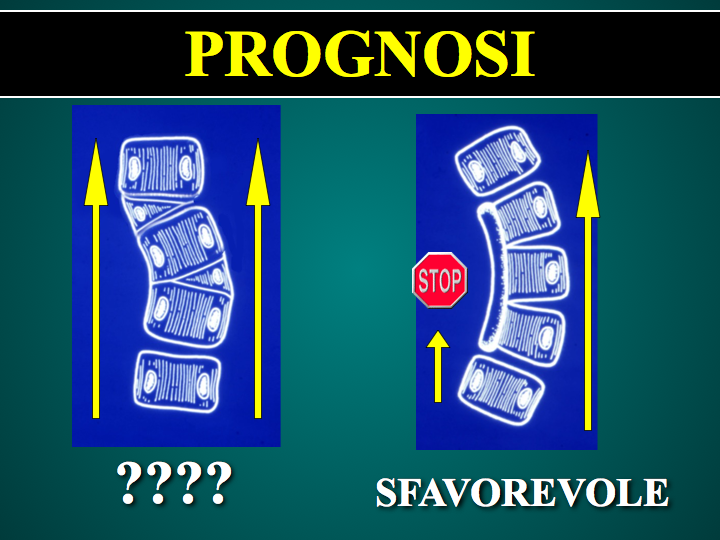
\includegraphics[width=0.5\textwidth]{012/image10.png}
\end{figure}

Questa distinzione è utile in termini di prognosi:

\begin{enumerate}
\def\labelenumi{\arabic{enumi}.}
\item
  Se ci sono 2 o 3 emispondili, questi possono crescere e
  \textbf{\emph{possono compensarsi}} l'uno con l'altro. In questo caso
  la colonna vertebrale più di tanto non si sposta con l'accrescimento
  dell'individuo e la prognosi non può essere predetta: devo monitorare
  la situazione durante l'accrescimento del bambino ed è possibile tale
  compensazione.
\item
  In caso di sinostosi il discorso sarà ben diverso dal momento che
  dalla parte in cui si ha la mancata segmentazione non vi è
  accrescimento e di conseguenza con lo sviluppo dell'individuo si avrà
  un \textbf{accrescimento asimmetrico} prevalentemente dalla parte che
  non presenta la fusione. In questo caso possiamo prevedere un
  \textbf{\emph{sicuro peggioramento}} con l'accrescimento del bambino.
\end{enumerate}

\paragraph{SCOLIOSI SECONDARIE }


Le scoliosi secondarie sono \textbf{dovute a malattie}:

\begin{enumerate}
\def\labelenumi{\arabic{enumi}.}
\item
  \textbf{Congenite} (ad esempio la neurofibromatosi, sindrome di
  Marfan, artrogriposi, la distrofia muscolare in cui viene meno il tono
  e la funzione muscolare).
\item
  \textbf{Acquisite} (ad esempio le \emph{\emph{idiopatiche}}, le
  \emph{poliomelitche}).
\end{enumerate}

Importante è una \textbf{diagnosi precoce}.

\begin{figure}[!ht]
\centering
	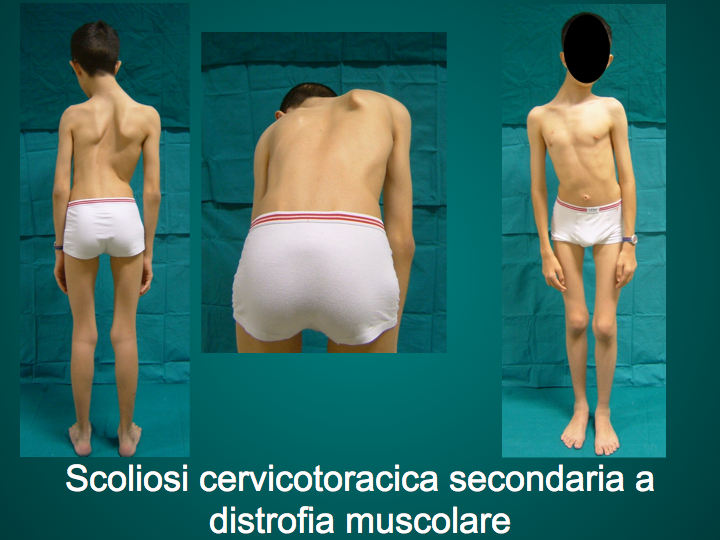
\includegraphics[width=0.5\textwidth]{012/image11.png}
\end{figure}
Nell'immagine è mostrata una scoliosi da \emph{distrofia muscolare}. Non si tratta di
una distrofia muscolare di Duchenne, ma probabilmente si tratta di una
\emph{sindrome del rachide rigido} (un'altra forma di miopatia)\emph{.}

La colonna vertebrale acquisisce delle curve molto gravi e anche il
torace ne risente (ne risentono anche i polmoni e gli altri organi del
mediastino: i dolori e l'artrosi sono il meno).

\begin{figure}[!ht]
\centering
	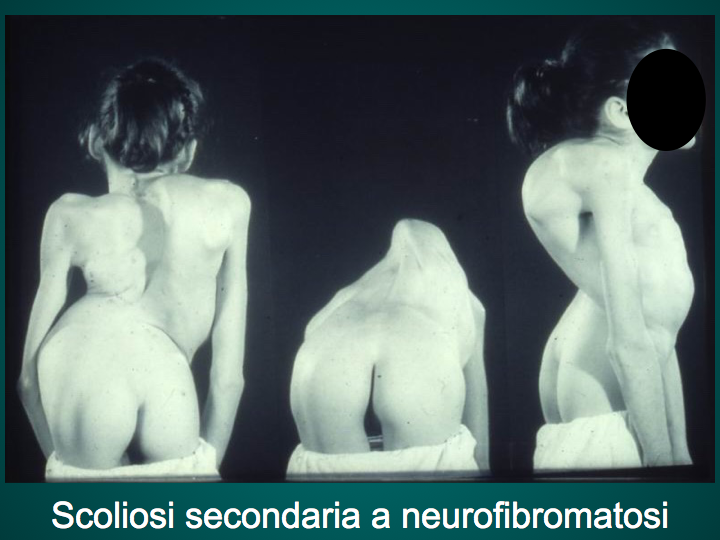
\includegraphics[width=0.5\textwidth]{012/image12.png}
\end{figure}

Scoliosi secondaria a \emph{neurofibromatosi}: la scoliosi si associa a
cifosi e si ha una cifoscoliosi. Si tratta di situazioni che ai nostri
giorni si vedono più raramente rispetto al passato.

\begin{figure}[!ht]
\centering
	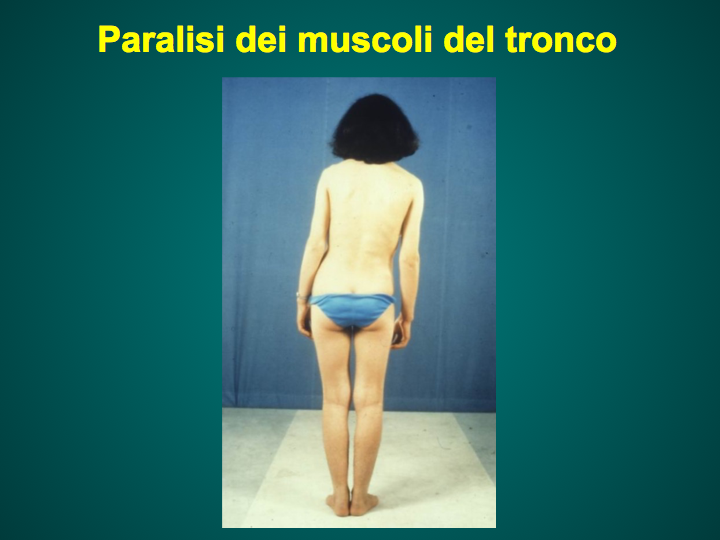
\includegraphics[width=0.5\textwidth]{012/image13.png}
\end{figure}
In una \emph{paralisi dei muscoli del tronco} (da qualsivoglia causa) la
situazione risulta molto meno impegnativa dal punto di vista ortopedico.

\paragraph{SCOLIOSI IDIOPATICHE}


Parliamo ora del gruppo delle scoliosi idiopatiche. Come suggerisce la
denominazione non se ne conosce la causa. Sono le scoliosi secondarie
più frequenti e generalmente compaiono in età giovanile o
adolescenziale. Tutta la partita si gioca dal momento in cui si fa la
diagnosi (che deve essere più precoce possibile) e da quel momento fino
a quando non si avrà la chiusura delle cartilagini di accrescimento (in
certe radiografie dovremo andare a vedere l'età ossea dell'individuo).
Evolvono in genere fino alla maturità ossea e terminato l'accrescimento,
termina anche la possibilità che la colonna vertebrale abbia un
peggioramento. \emph{IN REALTÀ} dopo la maturità ossea \textbf{\emph{non
ci può più essere ``\emph{peggioramento attivo''}}}: fenomeno in cui la
colonna cresce di più dalla parte della convessità e di meno dalla parte
della concavità. Però una volta che l'individuo ha terminato lo sviluppo
osseo, abbiamo una curva e quindi un'alterazione degli assi di carico e
\textbf{\emph{possiamo avere, in età adulta, un \emph{peggioramento}
chiamato ``\emph{passivo''}}} che non è dovuto a un accrescimento della
convessità, ma piuttosto a uno schiacciamento della concavità. Il
rapporto tra quantità di peggioramento attivo durante l'accrescimento e
la quantità di peggioramento passivo durante l'età adulta è nettamente a
sfavore del peggioramento passivo (lo schiacciamento è modesto rispetto
all'accrescimento che si ha nel peggioramento attivo). Di conseguenza
una scoliosi che a fine accrescimento è 25\textsuperscript{o}, a 60 anni può raggiungere i
30\textsuperscript{o}-35\textsuperscript{o} gradi. Ben diverso è l'aggravamento che può partire da 8\textsuperscript{o}-10\textsuperscript{o} in
età adolescenziale e può arrivare ai 50\textsuperscript{o} a fine accrescimento se non si
interviene per curare questa scoliosi (che è evolutiva).

Esiste una \textbf{classificazione topografica} di tali scoliosi. In una
radiografia possiamo individuare \emph{curve principali} e \emph{curve
secondarie} (la curva principale è quella che connota il tipo di
scoliosi: se parlo di scoliosi toracica significa che la curva
principale è completamente compresa nell'ambito del segmento toracico
del rachide).

In base alla localizzazione della \emph{curva principale} possiamo
distinguere le scoliosi in:

\begin{enumerate}
\def\labelenumi{\arabic{enumi}.}
\item
  \textbf{Cervico-toraciche;}
\item 
  \textbf{Toraciche;}
\item 
  \textbf{Toraco-lombari:} la curva principale è compresa sia nella
  parte toracica sia nella parte lombare della colonna\textbf{;}
\item 
  \textbf{Lombari:} la curva principale è compresa solamente nella parte
  lombare\textbf{;}
\item 
  \textbf{Doppie primarie:} sono dette anche \emph{\textbf{a ``S''
  italica}} perché su due curve non si riesce a capire quale sia quella
  principale: entrambe le curve presentano la stessa gravità e sono
  uguali per fenomeni di strutturazione cioè di rotazione. Sono le
  scoliosi di quelle persone che al colpo d'occhio dimostrano una
  lunghezza degli arti superiori eccessiva ( dipende dal fatto che se a
  livello del torace sono presenti 2 curve il torace sarà molto più
  corto e le braccia danno l'idea di essere più lunghe rispetto al
  normale)\textbf{.}
\end{enumerate}

\textbf{Scoliosi toraciche: }

\begin{enumerate}
\def\labelenumi{\arabic{enumi}.}
\item
  Si apprezza una \emph{gibbosità prevalente}. Il gibbo costale è dato
  dalla rotazione delle vertebre che si trasmette alle coste che
  deformandosi, deformano tutta la gabbia toracica. Quando la
  deformazione è eccessiva si hanno problemi polmonari e a livello del
  mediastino.
\item 
  Hanno una \emph{evoluzione spesso grave} (oltre i 30\textsuperscript{o} sono molto
  evolutive).
\item 
  A volte \emph{superano i 90\textsuperscript{o} con disturbi respiratori}. Questo è uno
  dei motivi per cui queste scoliosi vanno curate (o meglio non vanno
  fatte peggiorare). Il polmone dalla parte della concavità tende ad
  avere una insufficienza di tipo restrittivo con un aumento delle
  resistenze e il cuore destro inizia a faticare (si va verso quella che
  è la condizione del cuore polmonare cronico).
\end{enumerate}

\begin{figure}[!ht]
\centering
	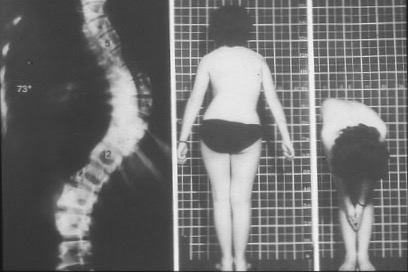
\includegraphics[width=0.5\textwidth]{012/image14.jpeg}
\end{figure}

Nella radiografia (scoliosi toracica) si apprezza la curva principale
(quella più grave). Nelle fotografie si vedono diversi segni come
l'asimmetria delle spalle e dei triangoli della taglia e il bacino che
ruota (esattamente come una vertebra). In flessione anteriore si vede
come la parte posteriore destra del torace sia assolutamente sporgente
rispetto all'altra parte (a dimostrazione della rotazione e quindi della
strutturazione). Se clinicamente non vediamo asimmetrie significa che la
scoliosi che abbiamo di fronte è una scoliosi finta (un atteggiamento
scoliotico).

La diagnosi viene sempre fatta con il malato sott'occhio e con la
radiografia: mai fidarsi di una cosa soltanto.
\\\\
Le \textbf{scoliosi toraco-lombari:}

\begin{enumerate}
\def\labelenumi{\arabic{enumi}.}
\item
  La curva principale in parte è nell'ambito del rachide toracico e in
  parte è nell'ambito del rachide lombare.
\item 
  Hanno una \emph{gibbosità molto marcata} che si apprezza quando il
  paziente si flette in avanti
\item 
  Hanno \emph{squilibri morfologici:} la persona risulta fuori asse
  rispetto alla superficie individuata dal bacino
\item 
  Sono \emph{molto evolutive} quindi, da un certo punto di vista, sono
  più soggette ad aggravamento.
\end{enumerate}

Le \textbf{scoliosi lombari: }

\begin{enumerate}
\def\labelenumi{\arabic{enumi}.}
\item
  Hanno \emph{salienze meno marcate} in quanto a livello lombare non
  sono presenti le coste. A parità di gravità più una curva è bassa e
  meno si vede. La rotazione delle vertebre lombari produce
  un'asimmetria chiamata \emph{\textbf{rigonfiamento lombare}} (non si
  parla di gibbo costale) ed è dovuto alla prominenza dei muscoli delle
  logge paravertebrali in seguito alla rotazione delle vertebre lombari
\item 
  \emph{Difetto estetico per differenza dei triangoli della taglia}
\item
  Sono abbastanza \emph{ben tollerate}
\item 
  Sono quelle che hanno una \emph{prognosi meno grave} (in realtà mai
  fidarsi di nessuno).
\end{enumerate}

Nella \textbf{scoliosi doppia primaria:}

\begin{itemize}
\item
  Non si riesce a capire bene quale sia la curva principale.
  Caratteristicamente si ha il torace un po' più corto e ciò fa sì che a
  colpo d'occhio le braccia possano sembrare molto più lunghe rispetto
  alla lunghezza del torace.
\item
  Le prominenze posteriori dal punto di vista clinico sono molto meno
  pronunciate.
\item
  Di solito clinicamente sono abbastanza ben compensate e non hanno
  tutti gli squilibri rispetto alle altre scoliosi.
\end{itemize}
\begin{figure}[!ht]
\centering
	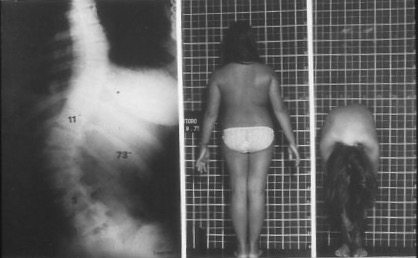
\includegraphics[width=0.5\textwidth]{012/image15.jpeg}
\end{figure}
\begin{figure}[!ht]
\centering
	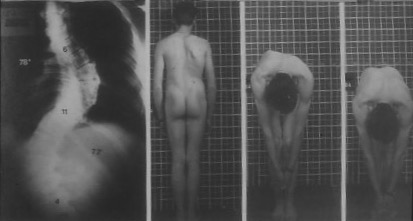
\includegraphics[width=0.5\textwidth]{012/image16.jpeg}
\end{figure}

Le curve scoliotiche più frequenti sono\textbf{:}

\begin{enumerate}
\def\labelenumi{\arabic{enumi}.}
\item
  Toraciche
\item 
  Toraco-lombari
\item 
  Doppie primarie
\item 
  Lombari
\item 
  Cervico-toraciche
\end{enumerate}

\subsubsection{Anatomia Patologica}

\begin{figure}[!ht]
\centering
	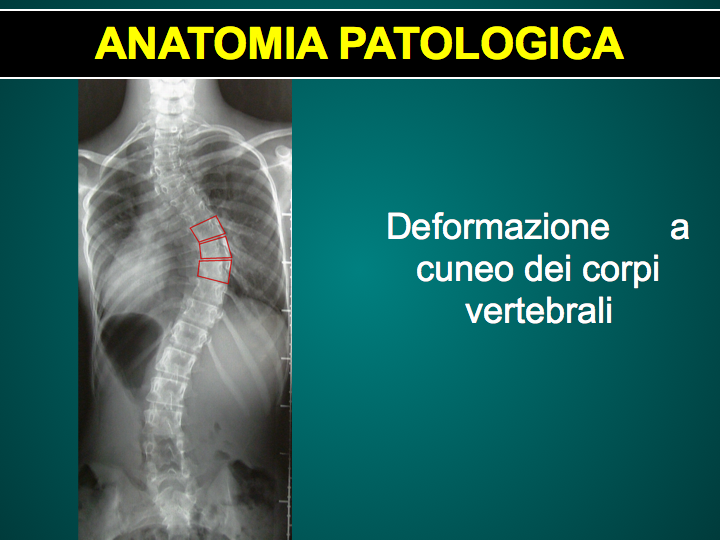
\includegraphics[width=0.5\textwidth]{012/image17.png}
\end{figure}
\begin{figure}[!ht]
\centering
	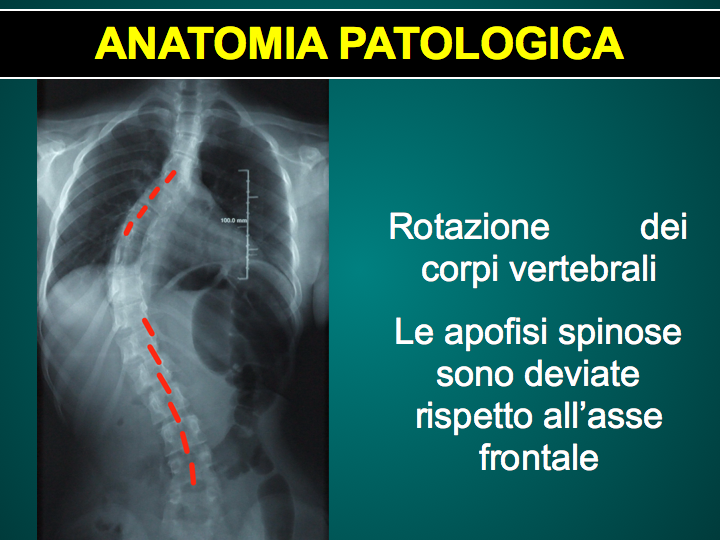
\includegraphics[width=0.5\textwidth]{012/image18.png}
\end{figure}
\begin{figure}[!ht]
\centering
	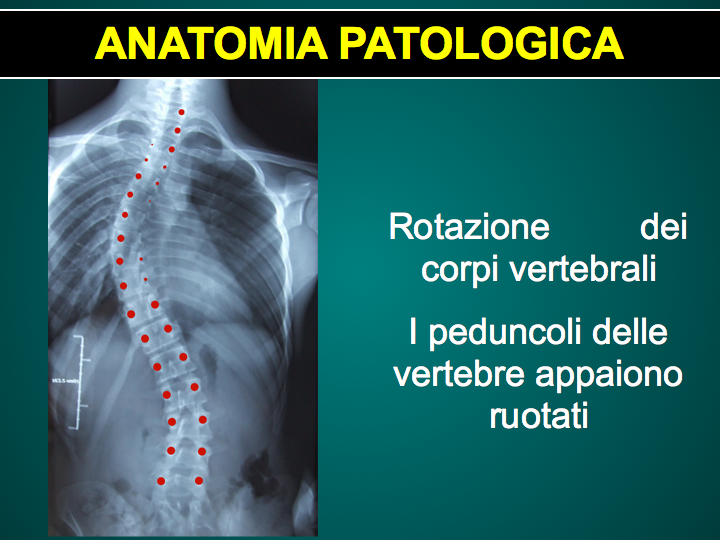
\includegraphics[width=0.5\textwidth]{012/image19.png}
\end{figure}
\begin{figure}[!ht]
\centering
	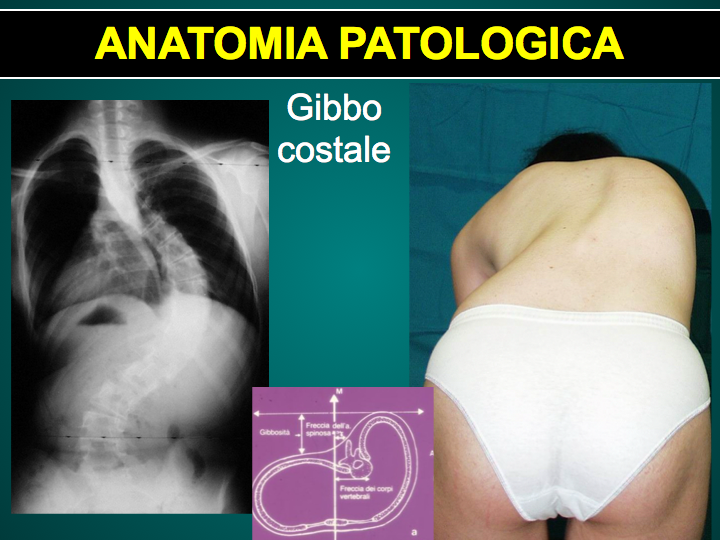
\includegraphics[width=0.5\textwidth]{012/image20.png}
\end{figure}

L'anatomia patologica è un'anatomia radiografica:

\begin{itemize}
\item
  \textbf{Deformità trapezoidale dei corpi vertebrali.} La deformità
  trapezoidale dei corpi vertebrali è uno dei fenomeni di
  strutturazione. Nella parte della concavità della curva c'è una
  riduzione dello spessore della vertebra mentre dall'altro lato la
  vertebra risulta più alta (si ha una deformità a cuneo o a trapezio
  dei corpi vertebrali).
\item
  \textbf{Rotazione dei corpi vertebrali.} Come si fa a vedere una
  rotazione dei corpi vertebrali? In una radiografia antero-posteriore
  del rachide si ha una proiezione diversa delle apofisi spinose
  rispetto al corpo vertebrale (visto come un rettangolo). La rotazione
  può essere vista anche attraverso la proiezione dei peduncoli
  vertebrali (i ``tondini'' nella diapositiva).
\item
  \textbf{Patogenesi del gibbo costale.} La rotazione vertebrale si
  trasmette alle coste e ciò si traduce in una modificazione della
  gabbia toracica. La modificazione non è solo di tipo estetico, ma è
  una modificazione anche di tipo funzionale perché si modifica lo
  spazio per il polmone.
\end{itemize}

\subsubsection{Clinica}


Il paziente deve essere svestito e viene valutato prima in stazione
eretta e poi lo si fa flettere in avanti mentre il medico è seduto e
alle spalle del paziente.

All'ispezione ciò che si vede è:

\begin{itemize}
\item
  Un'asimmetria \textbf{delle spalle}: una spalla più alta, l'altra più
  bassa
\item
  Un'asimmetria \textbf{delle scapole} non sono solo una più alta e
  l'altra più bassa, ma una è anche più spostata dal torace rispetto
  all'altra perché si ha una rotazione delle vertebre e quindi c'è gibbo
  costale
  \begin{figure}[!ht]
  \centering
  	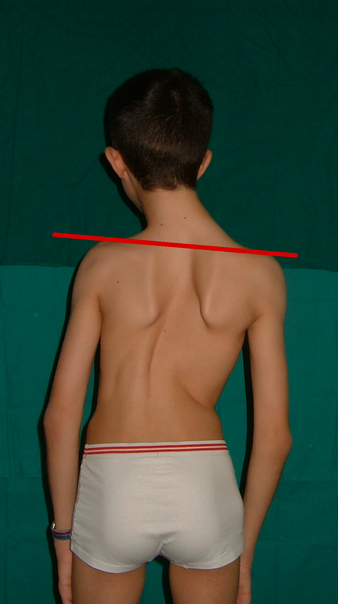
\includegraphics[width=0.3\textwidth]{012/image21.png}
  \end{figure}
\begin{figure}[!ht]
\centering
	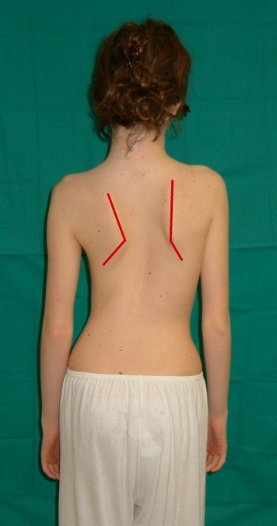
\includegraphics[width=0.3\textwidth]{012/image22.png}
\end{figure}
\begin{figure}[!ht]
\centering
	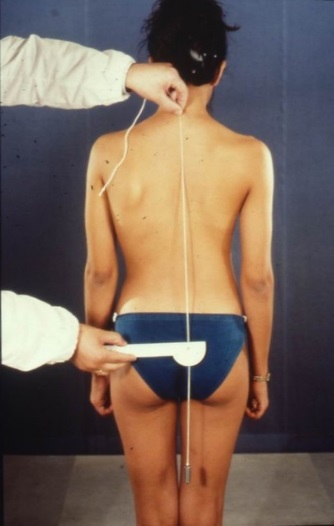
\includegraphics[width=0.3\textwidth]{012/image23.jpeg}
\end{figure}

\item
  Il \textbf{disassamento} che non è una costante, ma se presente è un
  evento prognostico sfavorevole. Lo si può valutare con un filo a
  piombo (ma generalmente basta un colpo d'occhio). Si applica il filo a
  piombo a livello della settima vertebra cervicale (C7, detta anche
  \emph{prominente}): in un rachide normale il filo a piombo dovrebbe
  cadere a livello del solco intergluteo mentre quando ho un
  disassamento (perché le \emph{curve secondarie non riescono a
  compensare completamente la curva principale)} si ha uno
  sbilanciamento e il filo a piombo non cade a livello del solco
  intergluteo. Il disassamento è un evento prognostico sfavorevole: se
  si riscontra disassamento è probabile che la curva peggiori proprio
  perché c'e questa incapacità da parte delle curve secondarie a
  compensare la curva principale.
\item
  Un'asimmetria \textbf{delle creste iliache}: i fianchi non sono
  uguali. Il bacino, ruotando sulle gambe, si comporta esattamente come
  una vertebra e si può pensare che il soggetto presenti un netta
  dismetria degli arti.
\item
  Un'\textbf{asimmetria dei triangoli della taglia} (triangoli
  delimitati lateralmente dal braccio e medialmente
  dal torace in alto e dal fianco in basso, il nome deriva dal fatto che
  le sarte prendono la taglia proprio da
  qui).
  \begin{figure}[!ht]
  \centering
  	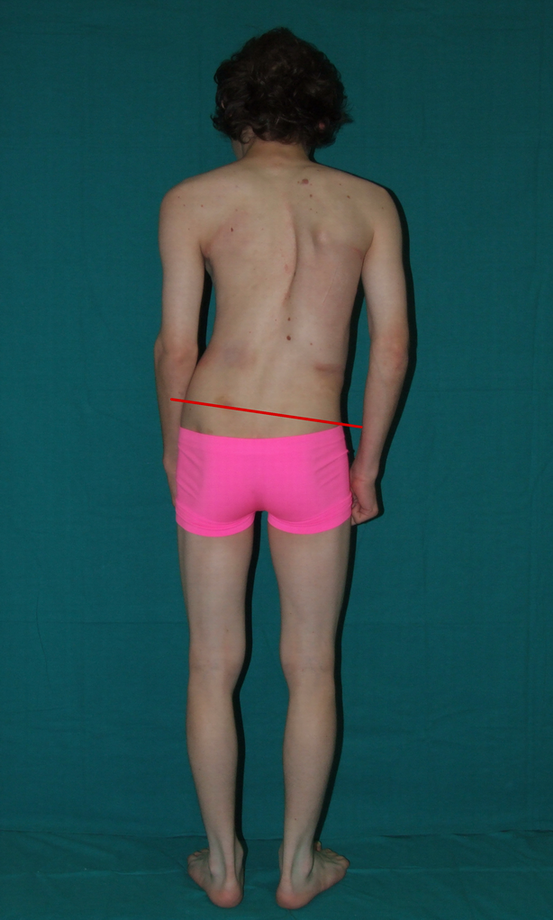
\includegraphics[width=0.2\textwidth]{012/image24.png}
  \end{figure}
  \begin{figure}[!ht]
  \centering
  	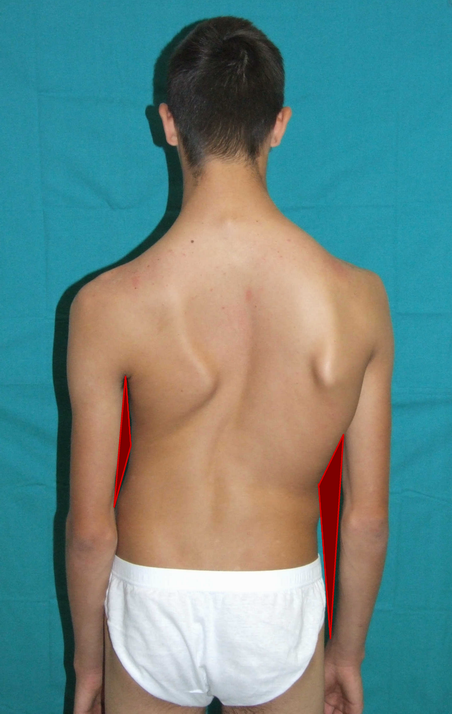
\includegraphics[width=0.2\textwidth]{012/image25.png}
  \end{figure}
  \begin{figure}[!ht]
  \centering
  	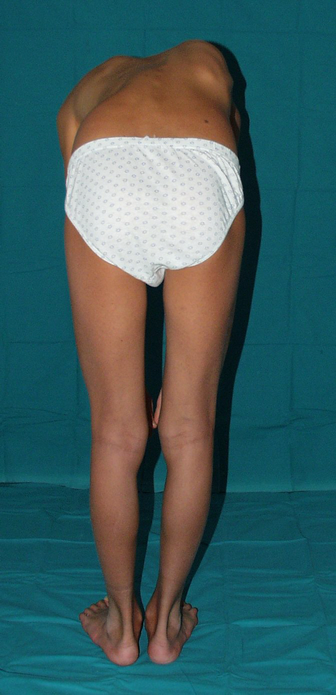
\includegraphics[width=0.2\textwidth]{012/image26.png}
  \end{figure}
  
\item
  Il \textbf{gibbo costale}: una volta che il paziente è stato esaminato
  in stazione eretta, da dietro, gli si chiede di piegarsi in avanti
  senza flettere le ginocchia (altrimenti si può falsare il tutto).


\begin{quote}
\textbf{N.B.In assenza del gibbo dobbiamo avere il dubbio che potrebbe
essere un atteggiamento e non una deformità vera.}
\end{quote}
\end{itemize}
\subsubsection{Studio radiografico}

La clinica va supportata dalla radiografia che ci serve anche per
cercare di capire se la scoliosi che ci troviamo davanti è una di quelle
poche che peggiorano o una di quelle molte che invece resterà tale.

La radiografia deve riguardare \textbf{tutta la colonna vertebrale} e
sarà in \emph{proiezione antero-posteriore} e durante la prima
osservazione anche in \emph{proiezione latero-laterale} (ci possono
essere delle modificazioni come una spondilolisi, che non si vedono in
proiezione antero-posteriore).

Radiografia panoramica del rachide in proiezione antero-posteriore e
latero-laterale sotto carico.
\begin{figure}[!ht]
\centering
	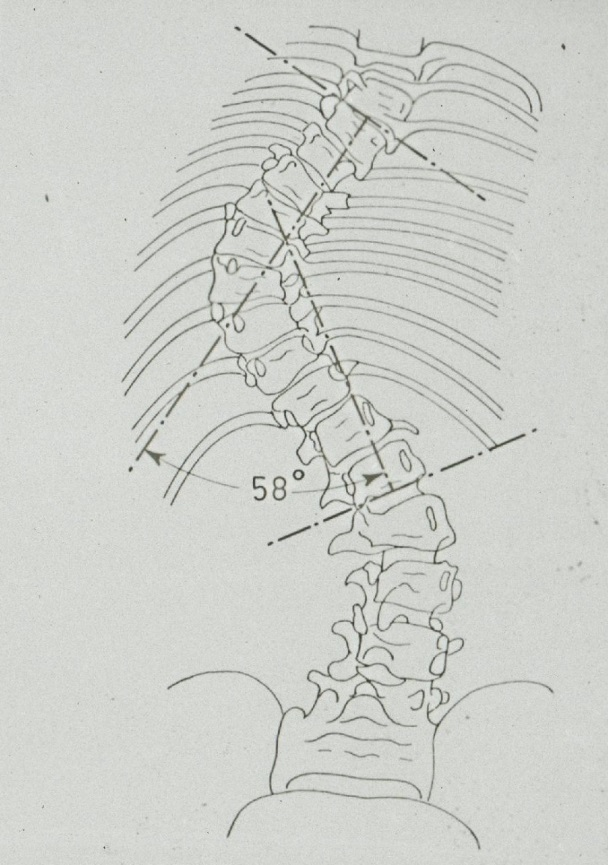
\includegraphics[width=0.4\textwidth]{012/image27.jpeg}
\end{figure}
\begin{figure}[!ht]
\centering
	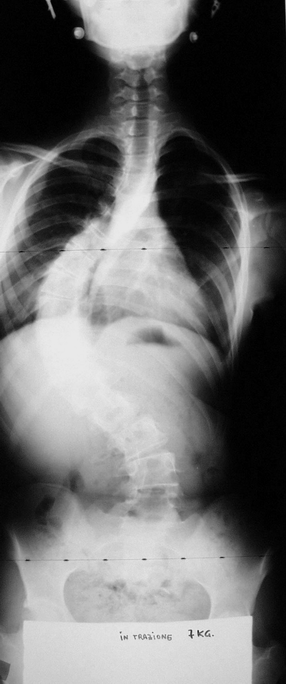
\includegraphics[width=0.1\textwidth]{012/image28.png}
\end{figure}
\begin{figure}[!ht]
\centering
	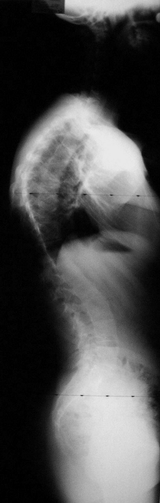
\includegraphics[width=0.1\textwidth]{012/image29.png}
\end{figure}

La radiografia deve comprendere anche le \textbf{ali iliache} perché è a
questo livello che è possibile studiare l'età ossea del bambino.

Nelle radiografie andiamo a ricercare:

\begin{enumerate}
\def\labelenumi{\arabic{enumi}.}
\item
  Dove si colloca la \emph{curva principale} ovvero la curva più
  importante, quella più grave, caratterizzata da fenomeni di
  strutturazione maggiori quindi i fenomeni di rotazione e deformità
  cuneiforme maggiori
\item 
  Valutiamo anche l'\emph{entità della curva} tramite la misurazione di
  Cobb (\textbf{metodo di Cobb})
\end{enumerate}

\textbf{Metodo di Cobb} per la \textbf{misurazione della curva.}
Consideriamo la curva toracica (nell'immagine). Si prende la vertebra di
confine superiore e quella di confine inferiore. Si traccia una tangente
al piatto SUPERIORE della vertebra SUPERIORE e una tangente al piatto
INFERIORE della vertebra INFERIORE. A questo punto si tracciano le
perpendicolari delle 2 rette individuate precedentemente (le due
tangenti) e si va a misurare l'angolo complementare individuato.

{[}In una curva come quella mostrata nell'immagine (abbastanza marcata)
le 2 rette (tangenti) possono convergere anche sulla radiografia (e
quindi la misurazione dell'angolo individuato potrebbe essere anche
abbastanza agevole). Se la curva fosse poco marcata, le 2 rette
tenderebbero a convergere a grande distanza (il professore dice che
``dovrei andare \emph{in giardino}'' per trovare la loro convergenza) e
quindi per semplificare la misurazione dell'angolo si ricorre alle
perpendicolari e alla misura dell'angolo complementare
(\emph{``\ldots{}questa si chiama geometria\ldots{}''}){]}.
\\\\
Altra cosa fondamentale per fare una prognosi è l'\emph{età: le}
scoliosi idiopatiche, come detto prima, peggiorano con l'accrescimento e
la possibilità di un peggioramento attivo termina con la fine
dell'accrescimento. È importante non tanto l'età cronologica del
soggetto, ma l'\textbf{età ossea} (età ossea ed età cronologica possono
non combaciare: ci sono bambini che si sviluppano prima e bambini che si
sviluppano dopo).

Una misura pura, in senso assoluto (\emph{``una scoliosi di 8\textsuperscript{o}''}), non
dice niente. Una scoliosi di 8\textsuperscript{o} in una bambina di 8 anni che deve ancora
andare incontro ad accrescimento è ben diversa da una scoliosi di 8\textsuperscript{o} in
una ragazza di 14 anni e mezzo già sviluppata da un anno e mezzo.
Perché? Perché si presuppone che la ragazza di 14 anni mezzo abbia meno
tempo per poter crescere ancora e quindi per poter peggiorare!

Il calcolo dell'età ossea viene fatto tramite il \emph{\textbf{TEST DI
RISSER}} \emph{valutando sempre la radiografia}: \textbf{si vanno a
studiare i nuclei di accrescimento delle ali iliache}\emph{.} Ci sono 5
o 6 stadi:

\begin{enumerate}
\def\labelenumi{\arabic{enumi}.}
\item
  \emph{Stadio 0} in cui non c'è nucleo
\item 
  \emph{Stadio 1} in cui comincia a comparire la parte laterale;
  progressivamente il nucleo tende a coprire le due ali iliache fino
  allo
\item 
  \emph{Stadio 3} in cui tutta l'ala è stata coperta, ma è ancora
  presente la cartilagine di accrescimento
\item 
  \emph{Stadio 4} in cui comincia a chiudersi la cartilagine di
  accrescimento in senso centrifugo, comincia a chiudersi la parte
  vicina alla colonna vertebrale {[}il nucleo cresce in senso centripeto
  mentre le cartilagini si chiudono in senso centrifugo{]}
\item 
  \emph{Stadio 5} in cui è completa la fusione e l'accrescimento è
  terminato.
\end{enumerate}
\begin{figure}[!ht]
\centering
	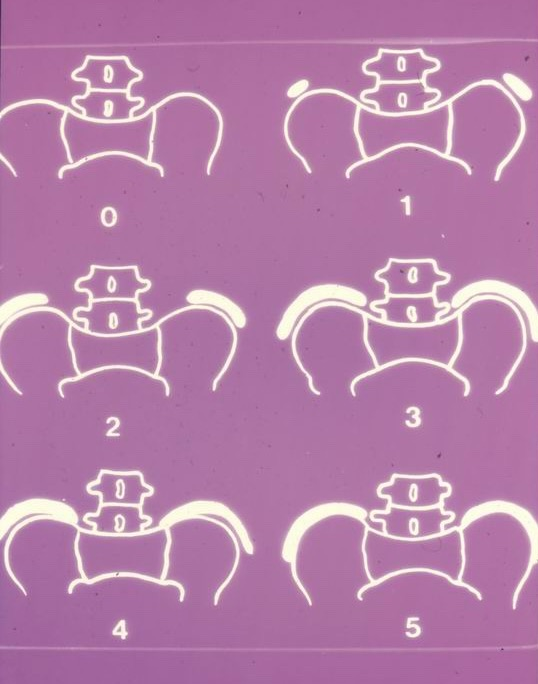
\includegraphics[width=0.5\textwidth]{012/image30.jpeg}
\end{figure}

Ciò è fondamentale per interpretare il numero che risulta dalla
misurazione di Cobb.

\subsubsection{Fattori di tipizzazione}


I parametri di cui si è detto sopra costituiscono i \textbf{FATTORI DI
TIPIZZAZIONE} e vengono di seguito riassunti:

\begin{enumerate}
\def\labelenumi{\arabic{enumi}.}
\item
  \textbf{EZIOLOGIA DELLA CURVA PRINCIPALE.} (Vedi quanto detto sopra)
\item
  \textbf{SEDE DELLA CURVA}. Nelle scoliosi idiopatiche c'è una
  differenza in base all'esperienza riguardo l'evolutiva della curva.
\item 
  \textbf{ENTITÀ DELLA CURVA}. Una scoliosi di 30\textsuperscript{o} al momento della
  diagnosi prima rispetto a una scoliosi di 8\textsuperscript{o}, ha subito bisogno di un
  trattamento on si aspetta tempo per vedere come evolverà la curva.
\item 
  \textbf{ETÀ CRONOLOGICA DEL PAZIENTE}.
\item 
  \textbf{ETÀ SCHELETRICA DEL PAZIENTE}.
\item 
  \textbf{STRUTTURAZIONE DELLA CURVA}. A volte ci sono curve lievi ma
  molto strutturate.
\item 
  \textbf{DISASSAMENTO.} È sempre un evento prognostico negativo.
\end{enumerate}

Tali fattori sono particolarmente utili nel caso delle scoliosi
idiopatiche dal momento che non si conosce la causa e permettono una
valutazione del quadro complessivo così da impostare il trattamento più
adeguato. Il grande problema delle scoliosi idiopatiche è che non si
conosce la causa e di conseguenza ci si deve ``arrampicare sugli
specchi''. Delle scoliosi ad esempio poliomielitiche sappiamo che
andranno incontro a peggioramento e di conseguenza verranno operate
prima che si inneschi la curva della colonna. Le scoliosi miopatiche
negli anni '90 venivano tutte operate (esperienza del professore):
veniva ``impuntellata" la colonna vertebrale perché si sapeva che tutte
le scoliosi sarebbero andate incontro a peggioramento. L'eziologia
dunque è fondamentale per il trattamento e anche per la prevenzione.

\subsubsection{Trattamento (delle scoliosi idiopatiche)}


Il problema in questo caso è individuare quelle che devono essere curate
che sono sempre una minoranza. Mettere il busto a tutte le scoliosi non
è la soluzione! Il busto è qualcosa di impegnativo. Immaginiamo di
mettere il busto a un bambino di 10 anni: il bambino dovrà andare a
scuola con il busto e ciò potrà avere un certo impatto psicologico su di
lui. A ciò si aggiungano le ripercussioni sull'assetto socioeconomico
della famiglia: ci sono famiglie che non capiscono e possono chiedersi:
perché devo curare qualcosa che non fa male? Di fatto nella scoliosi
idiopatica, ma più in generale \textbf{nella scoliosi giovanile},
qualunque sia l'eziologia, \textbf{non c'è mai dolore} e far capire a
una mamma che il figlio dovrà mettere un busto non è una cosa semplice.

Bisogna capire se ci si trova di fronte a una delle poche scoliosi
destinate a peggiorare o se è una delle molte che così sono e così
restano e che danno una colonna del tutto normale anche se magari non
perfetta, ma 8\textsuperscript{o} di scoliosi sono perfettamente compatibili con una vita
normale.

Non esistono a oggi lavori scientifici che dimostrino l'efficacia di
gran parte di quelli che vengono comunemente considerati (erroneamente)
trattamenti efficaci in queste forme di scoliosi come ad esempio la
ginnastica correttiva o sport come il nuoto (ci sono grandissimi
campioni di nuoto che praticano tale sport fin dall'adolescenza e che
comunque hanno delle scoliosi importanti.)

La \textbf{prevenzione non esiste}: la scoliosi, se vuole, si innesca o
peggiora indipendentemente da ciò che comunemente si sente dire
funzioni.

A questo punto il prof si sofferma su alcuni luoghi comuni come quello
che definisce il mito degli sport asimmetrici quali il tennis: non
esistono evidenze che dimostrino che gli sport asimmetrici possano
innescare o peggiorare una scoliosi. Il corpo umano è naturalmente
asimmetrico (la maggior parte di noi è destrimane mentre la minoranza è
mancina ed è ovvio che il nostro corpo non è simmetrico).

Altro luogo comune è quello dei materassi duri: anche in questo caso non
ci sono evidenze scientifiche.

Quando il professore era specializzando si partiva dal presupposto che
si potessero stimolare i muscoli dalla parte della convessità perché
dalla parte della concavità i muscoli erano più forti. Con
l'elettrostimolazione si cercava di stimolare questi muscoli, ma i
risultati ottenuti sono stati del tutto negativi.

Trattamento della scoliosi (sintomo):

\begin{enumerate}
\def\labelenumi{\arabic{enumi}.}
\item
  Diagnosi precoce
\item
  Controllo evolutivo
\item 
  Trattamento ortopedico
\item 
  Trattamento chirurgico
\end{enumerate}
